\documentclass[12pt]{article}

\newlength\tindent
\setlength{\tindent}{\parindent}
\setlength{\parindent}{0pt}
\renewcommand{\indent}{\hspace*{\tindent}}

%% packages
\usepackage{enumerate}
\usepackage{listings}
\usepackage{multicol}
\usepackage{amsmath}
\usepackage{caption}
\usepackage{subcaption}
\usepackage[a4paper,margin=2cm]{geometry}
% \usepackage[english, norsk]{babel}
\usepackage{fancyhdr}
\usepackage{pdfpages}
\usepackage{lastpage}
% \usepackage[demo]{graphicx}
\usepackage{graphicx}
\graphicspath{ {.} }


\date{}
\begin{document}

% intentionally empty
\author{Faculty of Mathematics and Natural Sciences}

\title{UNIVERSITY OF OSLO}

\maketitle 
\begin{center}
\textbf{Exam in GEO4300/GEO9300 -- Geophysical Data Science}
\end{center}


Day of exam: 28 November, 2018 \\
Exam hours: 14:30 -- 17:30 (3 hours) \\ 

This examination paper consists of \pageref{LastPage} pages including this page and appendices. \\

Permitted materials: calculator\\ 

Note: \\
1. This examination paper has to be returned together with your answers/solutions.\\
2. This exam is a closed book exam. Only a calculator is permitted.\\ 
3. Make sure that your copy of this examination paper is complete before answering.\\ 
4. There are in total 50 points in this exam.\\


\pagebreak

\section{Probability density function}
The probability density function of a random variable $x$ is given as:

$$ f(x)=\frac{1}{\sqrt{2 \pi \sigma^2}} e^{- \frac{(x-\mu)^2}{2 \sigma^2}} $$

\begin{enumerate}[(a)] 
\item Draw a free-hand figure to illustrate the density function and indicate on the figure the probability $prob(x<a)$, $prob(a<x<b)$ and $prob(x>b)$ \textbf{\hfill (3 points)}
\item Draw a free-hand figure to illustrate the cumulative probability distribution function and indicate on the figure the probability $prob(x<a)$,  $prob(a<x<b)$ and $prob(x>b)$. \\ \textbf{\hfill (3 points)}
\item Define or explain the first and second moment of $x$. \textbf{\hfill (4 points)}
\end{enumerate}


%\pagebreak
\section{Frequency analysis and linear regression}
\begin{enumerate}[(a)]
\item What is the probability to observe at least one 200-years flood or larger within a period of 10 years? \textbf{\hfill (5 points)}
\item Figure 1A shows a simple linear regression between average runoff and median annual flood. Figure 1B shows the QQ-plot of the residual where the theoretical quantiles were calculated using the normal distribution. Describe which assumption of a simple linear regression is violated in this analysis, and discuss strategies that can be used to improve the analysis. \textbf{\hfill (5 points)}
\end{enumerate}

\begin{figure}[h!]
    \centering
    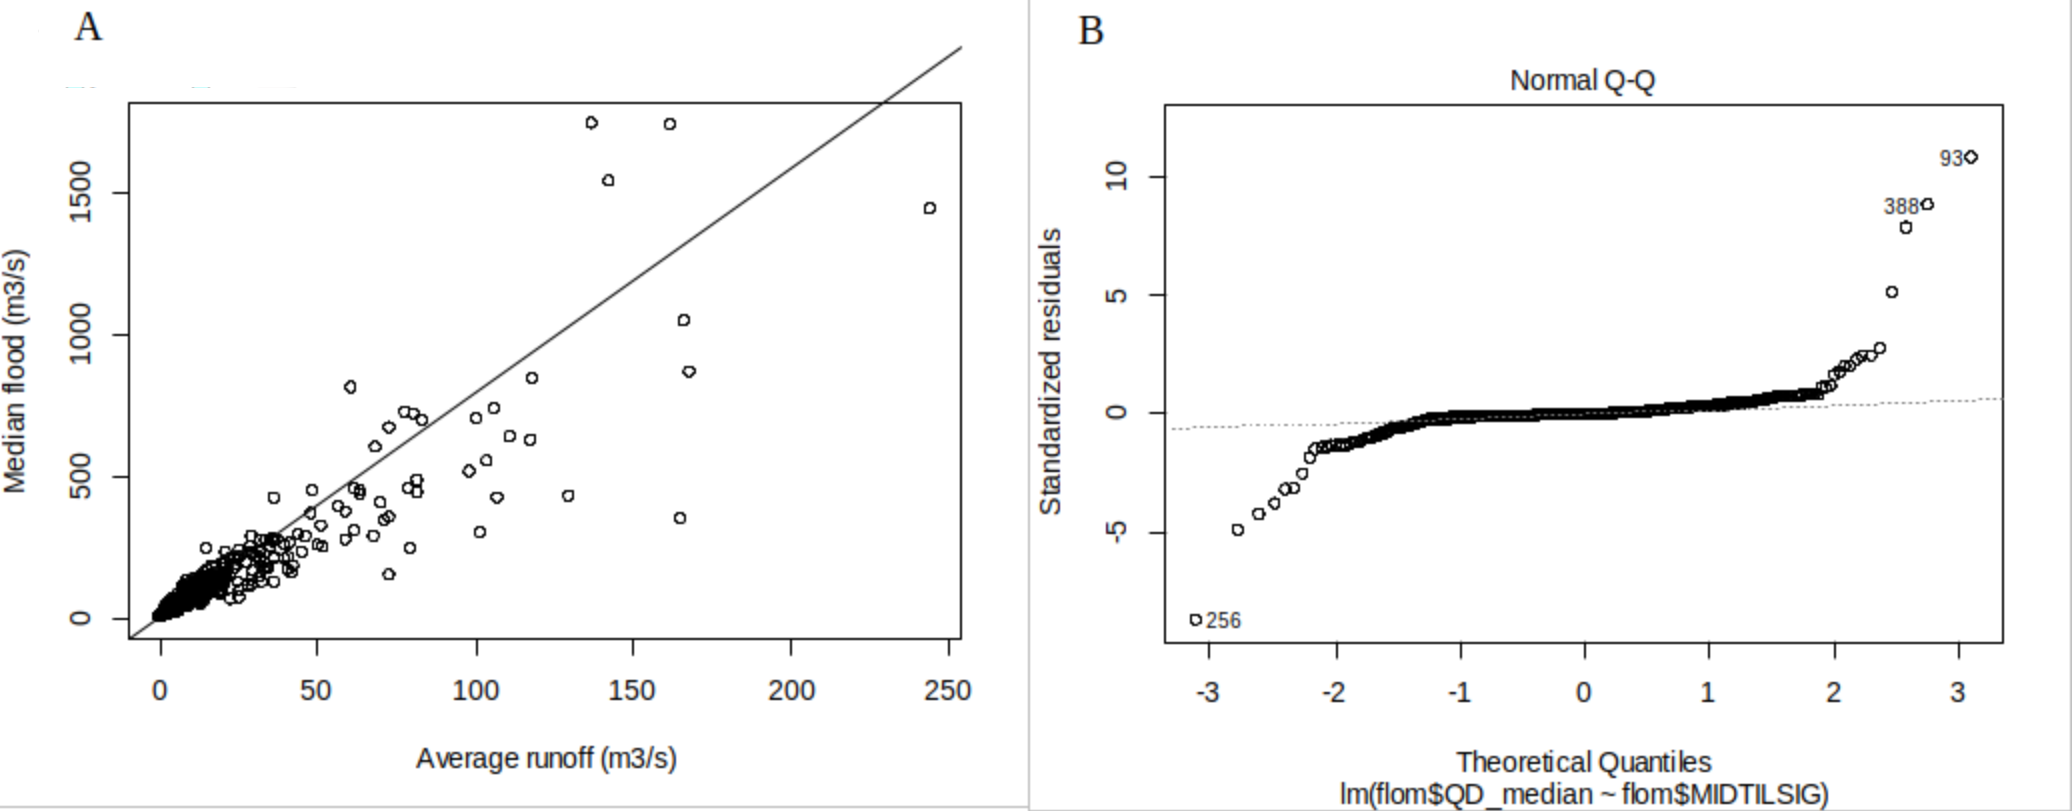
\includegraphics[width=.8\textwidth]{fig01} 
    \caption{A) linear regression, B) Q-Q plot.}
\end{figure}


%\pagebreak
\section{Hypothesis testing}
Below is a 20-year dataset (all values are in m$^3$/s) with observations of runoff before a human intervention, and a 7-year dataset from after the human intervention in a basin. \\

Before the intervention:\\
24, 12, 48, 17, 14, 28, 11, 13, 31, 34, 34, 12, 48, 14, 28, 17, 11, 13, 31, 24 (mean = 23.2, standard deviation = 11.48)\\

After the intervention:\\
29, 46, 49, 31, 28, 50, 31 (mean = 37.7, standard deviation = 9.32)\\


Could it be stated from this small sample that the runoff (both mean and variance) was affected by the intervention? Use a significance level of 5\%.

\textbf{\hfill (10 points)}


%\pagebreak
\section{Goodness-of-fit testing}
Based on 90-year records of yearly maximum discharge ($Q$ in m$^3$/s) at two adjacent stations, the following statistics are calculated (with $n=90$):

\begin{table}[h!]
\begin{tabular}{l|c|c|c|c|c}
& $Q \le 50$ & $50<Q \le 100$ & $100<Q \le 150$ & $150<Q \le 250$ & $Q>250$ \\
\hline
Station A (\# years) & 6 & 24 & 35 & 15 & 10 \\
Station B (\# years) & 5 & 25 & 20 & 26 & 14 \\
\hline
\end{tabular}
\end{table}

The mean value in station A is 130 m$^3$/s, standard deviation in A is 5 m$^3$/s.
The mean value in station B is 120 m$^3$/s, standard deviation in B is 5 m$^3$/s.

\begin{enumerate}[(a)] 
\item Sketch the cumulative histograms of the two datasets in the same plot and describe the characteristics of the distributions. \textbf{\hfill (5 points)}
\item Use the Chi square method to test the hypothesis that data in Station A and Station B have the same distribution. Use a significance level of 5\%. \textbf{\hfill (5 points)}
\end{enumerate}


%\pagebreak
\section{Time series analysis}
\begin{enumerate}[(a)]
\item What is meant by second-order stationarity in a time series? \textbf{\hfill (5 points)}
\item How could you test for a trend in a time series? Explain a suitable test. \textbf{\hfill (5 points)}
\end{enumerate}


%\pagebreak
\section{Appendix: Formulary}

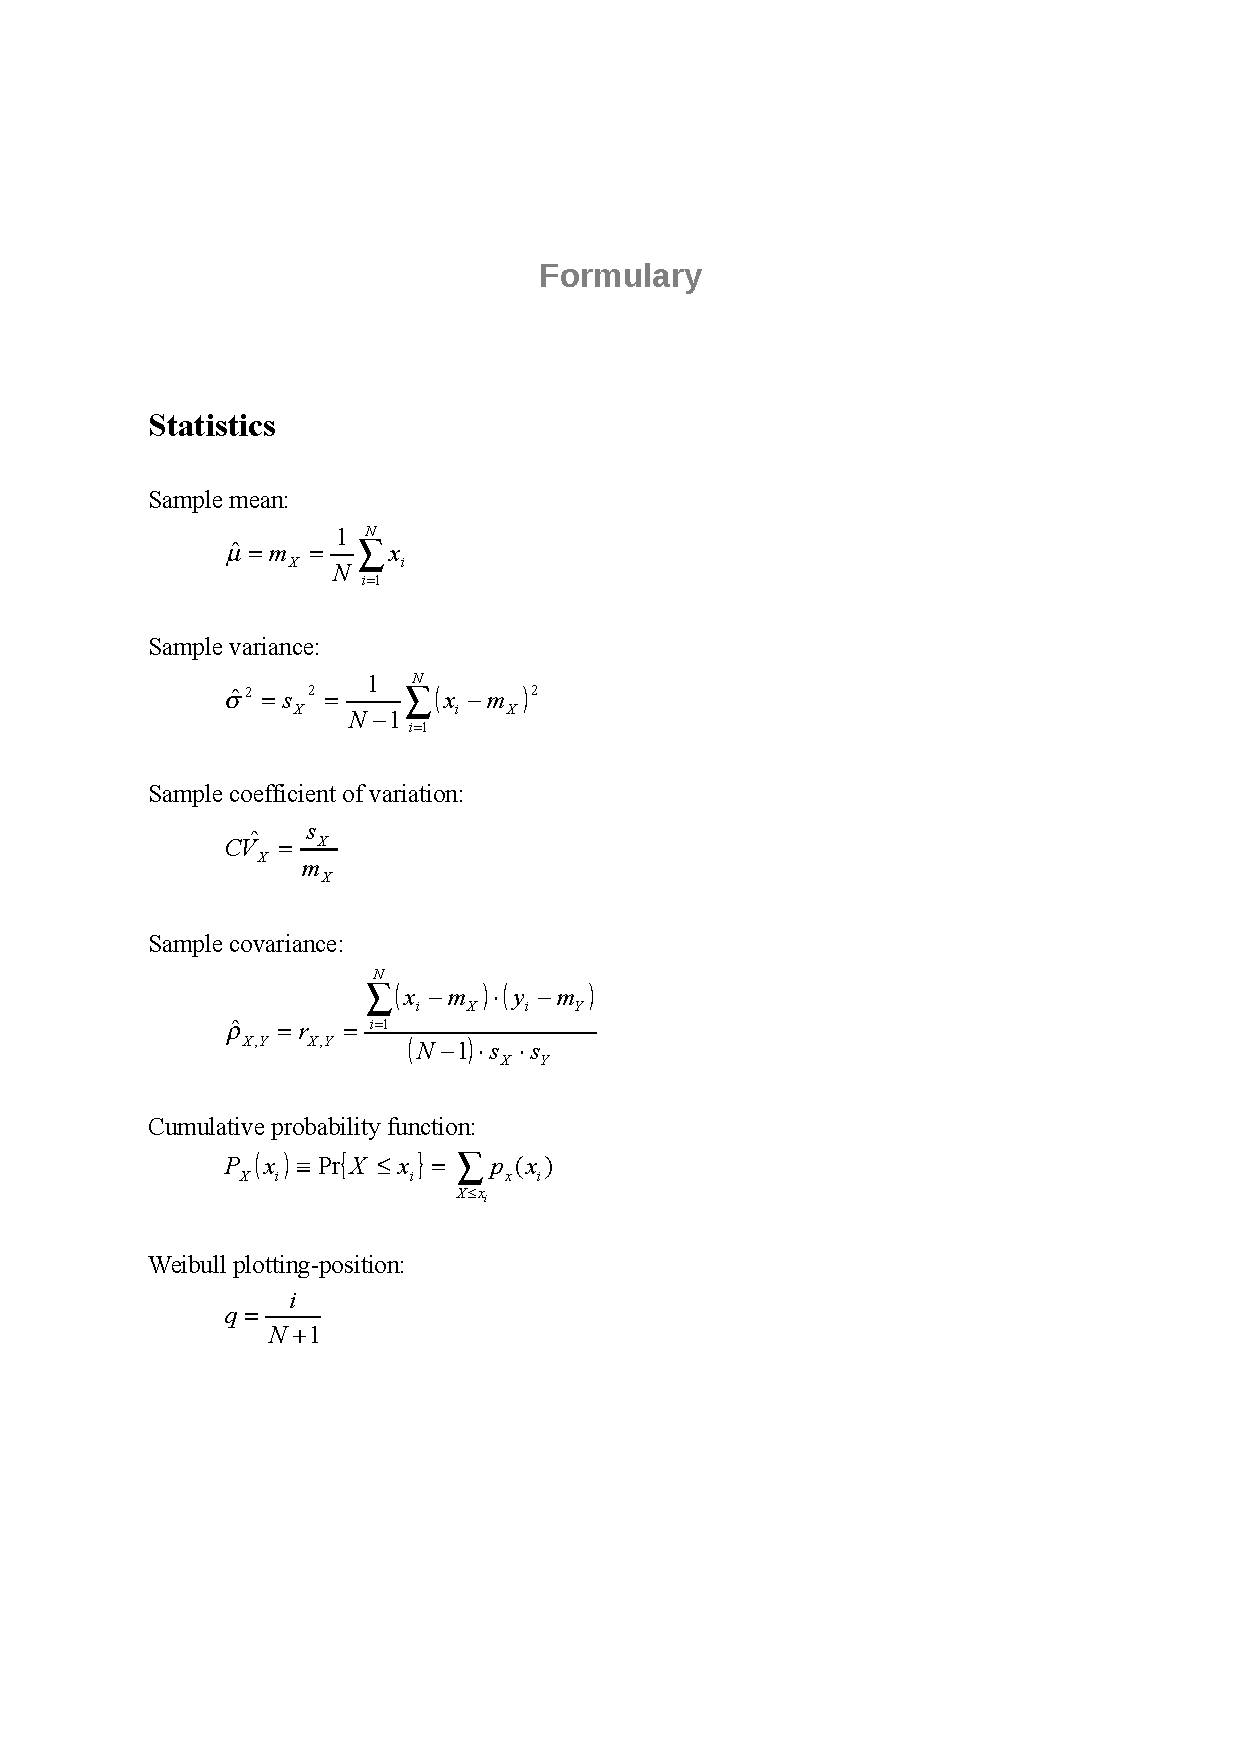
\includepdf[pages={1-12}]{formulary-2017_final.pdf}


\end{document}











